
\subsection{Einleitung}
Hauptursache für diese Problematik ist die oft unverschlüsselte, zentrale
Speicherung der Daten. Damit aber nicht auf den Komfort verzichtet werden muss,
der von üblichen Dateisynchronisationsdiensten geboten wird, werden die zuvor angesprochenen
Probleme bei \sblit umgangen.

Bei \sblit werden Dateien anstatt über einen Server, nämlich über verschlüsselte
\glspl{p2plink} zwischen zwei Endgeräten direkt übertragen.
Oft kommt es allerdings vor, dass \glspl{syncpartner} beim Verändern von
Dateien nicht erreichbar sind und kein \gls{p2plink} aufgebaut und auch
keine Datei synchronisiert werden kann.
Mit dem Senden einer neuen Version von Dateien zu warten,
bis beide Clients gleichzeitig erreichbar sind, hätte eine zu große Zeitspanne
zur Folge, in der viele Versionskonflikte auftreten könnten.
Deshalb verwendet \sblit eine Cloud, um Dateien für nicht erreichbare
Synchronisationspartner extern zwischenspeichern zu können. Die Cloud bildet
sich dabei aber nicht aus einem Server, wie üblich, sondern aus einem \gls{p2pnet}
aller Nutzer von \sblit. Diese dezentrale \gls{filecloud} wird
mit sogenannten \glspl{partnership} realisiert. Dabei geht es darum, dass sich
User, die sich gegenseitig nicht kennen müssen, einander ihre Daten direkt über
verschlüsselte Kanäle auf den Geräten des jeweiligen anderen speichern.
Um die Dateien nicht nur sicher zu übertragen, sondern auch zwischenzuspeichern
ohne, dass Dritte Zugriff haben, werden die zu
synchronisierenden Dateien in Blöcke aufgeteilt und verschlüsselt. Diese
verschlüsselten Blöcke werden dann verteilt auf die Partnergeräte gespeichert,
sodass diese fremden User nichts damit anfangen können, da sie weder den
Schlüssel zum Entschlüsseln, noch die Informationen über den Ort der restlichen
Blöcke besitzen. Diese befindet sich ausnahmslos nur bei dem User, zu dem die
Blöcke gehören.

\subsubsection{Szenario}
Bei \sblit wird der Inhalt eines Ordners synchronisert, der bei der
Konfiguration angegebenen wurde. Sobald sich Dateien innerhalb des Ordners
ändern, wird die neue Version der Datei kopiert und die Kopie wird den
erreichbaren Synchronisationspartnern über einen \gls{p2plink}
gesendet.

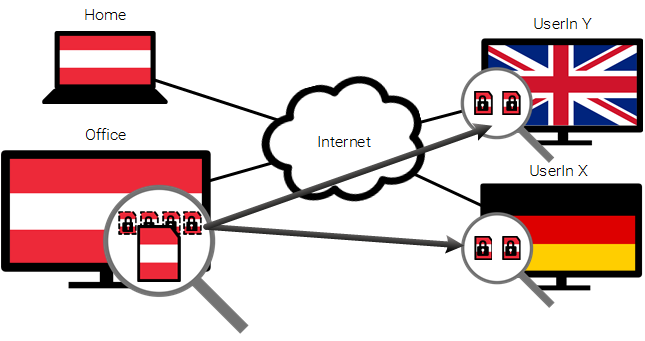
\includegraphics[]{images/sblit_1}
Übertragung der Datei zwischen zwei erreichbaren Hosts.

Für Synchronisationspartner, die nicht erreichbar sind, wird die Datei in der dezentralen
\gls{filecloud} zwischengespeichert. Die Datei wird kopiert und in Blöcke
aufgeteilt. Diese Blöcke werden mit dem privaten Schlüssel des Clients
verschlüsselt und verteilt auf den \glspl{partnerdevice} gespeichert.

Da die Erreichbarkeit der Partnergeräte, auf denen die veschlüsselten
Datei-Blöcke gespeichert sind, nicht gewährleistet ist, wird die Datei mehrmals
in die dezentrale \gls{filecloud} gespeichert, sodass nur ein Bruchteil der
Partnergeräte erreichbar sein muss, um auf die vollständige Datei zugreifen zu
können.

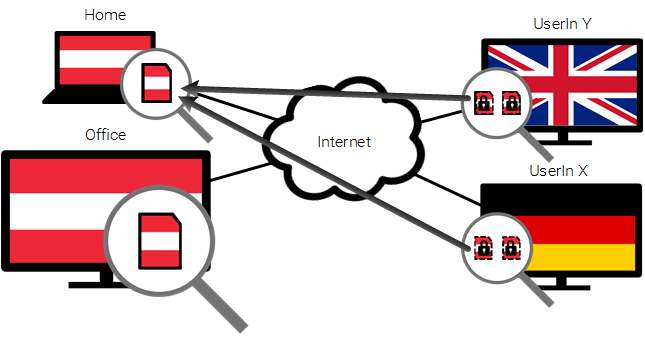
\includegraphics[]{images/sblit_2}
Hochladen der Datei in die dezentrale \gls{filecloud}.

Sobald der Synchronisationspartner, hier Home_1 wieder erreichbar, also dem
\gls{p2pnet} beigetreten ist, fordert er die verschlüsselten
Dateiblöcke von den \glspl{partnerdevice} an. Verschlüsselte \glspl{p2plink}
werden aufgebaut und die Blöcke werden übertragen, entschlüsselt und zu der
vollständigen Datei zusammengesetzt.

Die Datei wurde also über die Partnergeräte synchronisiert, die eine dezentrale
\gls{filecloud} darstellen.

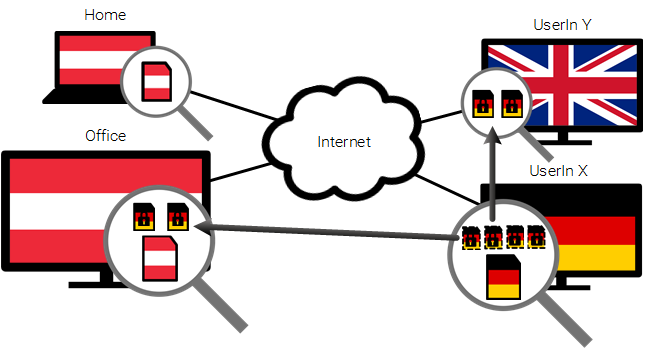
\includegraphics[]{images/sblit_3}
Gegenseitiges Speichern von Dateiblöcken (Konzept einer \gls{partnership}).

Im Gegenzug, dass man Daten auf Geräten anderer speichern darf, gibt man selbst
Speicherplatz für diese User frei, in dem die von ihnen verschlüsselten
Dateiblöcke zwischengespeichert werden können. Der für andere User freigegebene
Speicherplatz beträgt dabei die Speichermenge, die man selbst bei anderen Usern
beansprucht.
